\documentclass[12pt]{report}

\usepackage[utf8]{inputenc}
\usepackage[english]{babel}
\usepackage{graphicx}
\usepackage[pdf]{pstricks}

%Options: Sonny, Lenny, Glenn, Conny, Rejne, Bjarne, Bjornstrup
%\usepackage[Sonny]{fncychap}
\usepackage{amsmath}
\usepackage[colorlinks=true, allcolors=blue]{hyperref}
\usepackage{hyperref}
\usepackage[a4paper,top=3cm,bottom=3cm,left=3cm,right=3cm]{geometry}

\graphicspath{ {imgs/} }

\title{
  {\Huge Inferring program structure from an execution trace}
}
\author{
  {Juan Francisco Martínez Vera}\\
  {\tt juan.martinez@bsc.es}
}
\date{\today}

\begin{document}
\maketitle
\tableofcontents

\chapter{Introduction}
A typical configuration for high performance machines are clusters. It means a t
eam of individual processors or multiprocessors (and lately more specific hardwa
re like GPUs) working together, interconnected by a super-fast network. The fund
amental idea behind these big machines is getting speedup by mean of partitionin
g the problem and parallelize the execution. So all processors (or a subset) in 
the cluster will be dealing with different parts of the same problem and communi
cating between them in order to end up with a solution. For example imagine we h
ave a weather forecast software, in order to speedup the forecast we can partiti
on the surface of the earth and hold every portion to one individual processor. 
The communication will be needed because the weather will also depend on surroun
dings, so every partition will need also information of other partitions results.

In Computer Science the discipline in charge to drive research in this field is 
the High Performance Computing, i.e. HPC. HPC has been increasing in importance 
and nowadays can be said it is the third support of science with theory and math
ematics. The science that can be done thanks to this big machines goes from eart
hquake predictions to the analysis of the DNA of a carcinogenic cell, from weath
er forecast to material physics simulation. HPC research is not just limited to 
the hardware layer but drive research in all layers in the Transformation Hierar
chy\cite{transformationHierarchy} in figure \ref{transformationHierarchyImg}.

\begin{figure}
  \caption{Levels of transformation}
  \label{transformationHierarchyImg}
  \centering
    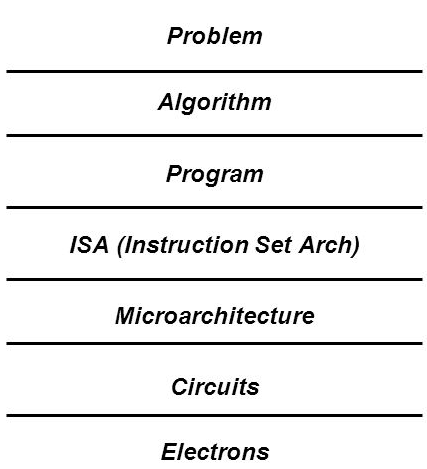
\includegraphics[width=120px]{transformationhierarchy.png}
\end{figure}

\begin{figure}
  \caption{Gordon Moore's prediction done in 1965}
  \label{moore-prediction}
  \centering
    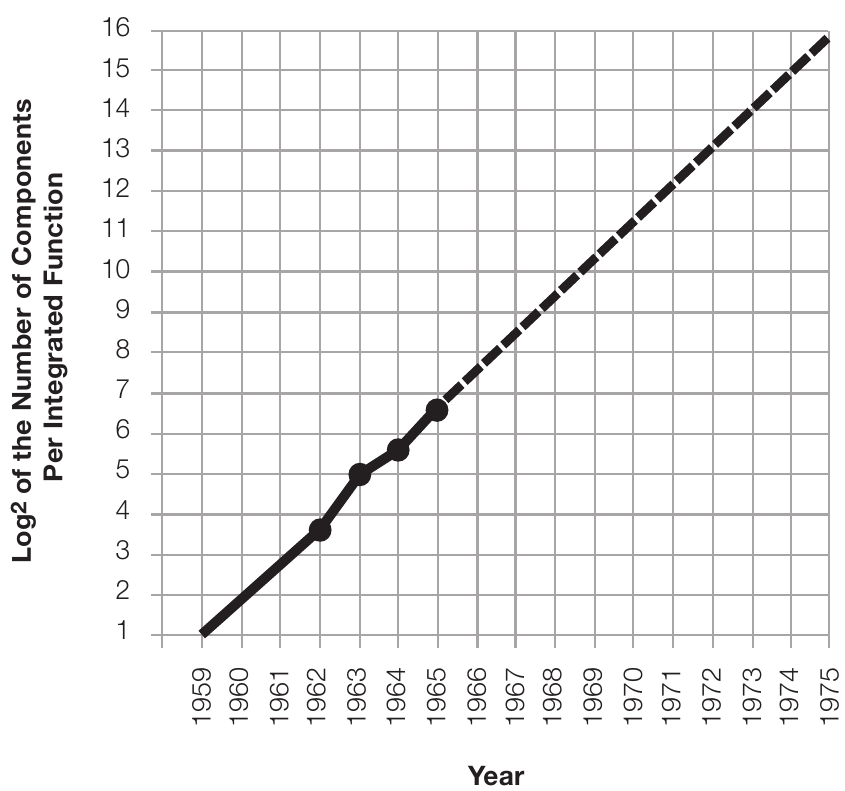
\includegraphics[width=200px]{moore_prediction.png}
\end{figure}

Resources are limited and expensive, so we have to be smart and use them in an
efficient way. Improving the efficiency is not just a matter that affects to one
layer of the stack but can be applied to every one of them. For example the
tremendous evolution of the last fourty years were improvements done mostly on
circuits layer what have been following the Moore's law \cite{moore:1965}. The
manufacturers have been reducing the size of transistors by a ration of 2 every
18 months as were predicted in figure \ref{moore-prediction}. Performance improvements 
were also at microarchitecture level with
disruptive designs that allows ILP like HPS\footnote{High Performance Substrace,
what is indeed out-of-order execution with in-order retirement.}
\cite{Patt:1985:HNM:18927.18916}, speculative execution with prefetchers, 
branch prediction or even memory access value speculation,
VLIW\footnote{Very Long Instruction Word} or TLP\footnote{Thread Level
Parallelism} with multi-threading. Improvements on memory hierarchy like cache 
associativitym, non-blocking cache or trace cache. The last
big revolution affected both architecture and program layers and was the 
multicore revolution. Was specially important because until then, programmers were 
agnostics, just feel their programs went faster but now, programs have to be 
architecture aware. With this last revolution a new effort for hide machine stuff
from programmers arise and end up with programming models like OpenMP
\cite{openmp_new}, OpenACC\cite{openacc_new} or OmpSs\cite{ompss_new}. A relatively
recent example is shown is this paper \cite{Alvarez:2015:CPT:2872887.2750411}
where they are trying to automatically use the fast scraptchpad memories by
means of compilers procedures and extra hardware support instead
of let programmers to deal with this piece of hardware directly. The need to be 
always faster and faster is even more pressing in HPC that is in fact an
important science driver.

This thesis is centered on program layer\footnote{The program layer 
bring together the program itself, programming models, frameworks and libraries.}. 
This layer is the actual implementation of the algorithm, i.e. where programmers
transforms algorithm to  semantic code that can be transformed lately into
executable binary by compilers. This layer is indeed the interface between pure 
algorithm and the machine architecture. Having an efficient algorithm
mathecamically speaking is not enforcing having an efficient program 
because at algorithm level we do not care about the machine. 
The mechanism to assess the quality in terms of performance are the {\bf performance 
analysis tools} that allows to analyze and detect the bottlenecks. 
There are two main trends, by one hand we have the profilers and by other hand trace
tools. Profiler tools provide performance summaries. This summaries provides 
coarse-grain information, with low-overhead. It means that you can feel the problem 
and infer what could be the origin but the information is not enough if you want 
to be sure. For gather more detail, the other typical approach are the tracing 
tools. High accurate and detailed information can be obtained, but it needs 
more resources in terms of cpu, disk and analyst effort because more data implies 
more complexity. This demand of resources becomes worst since the capacity in 
terms of parallelism is increasing, so the number of tasks to monitor makes 
tracing by one hand hardly scalable and by the other hand tricky to analyze
because the huge quantity of data and because the increasing response times
during the interactive exploration of analysis results. 

Researchers are currently facing this two drawbacks. There are currently several
specialists driving research in the scalability field, they are trying to reduce 
the overhead of tracing in terms of time and trace sizes by mean of several 
techniques like machine learning, data-mining and so on like in 
\cite{llort2015intelligent} or by on-line compression like in
\cite{noeth2009scalatrace}. About analysis field, the complexity of the analysis 
can be overcome by adding intelligence to performance analysis tools, last 
trend is to provide an automatic smart layer that automate an important part 
of the analysis and help the analyzers in their work. Some examples of this 
research line are automatic performance analysis \cite{wolf2003automatic}, 
automatic structure extraction \cite{casas2007automatic}, phases detection 
\cite{gonzalez2013application} fundamental factors models \cite{casas2008aass}, 
automatic analysis throw deep learning \cite{simon:2017:perfdp} and so on.

This thesis is focused on the analysis field and is devoted to humbly contribute 
to ease the work of the analyzers by
automate part of the analysis. The goal of this work is to automatically detect
the internal structure of an application and correlate it with performance metrics by
mean of a post-mortem trace analysis that will help analyzers to have a general
overview about what is actually going on. So instead of deal with whole
information from the very beggining, this approach let the analyzer to figure
out to what part of the gathered information focus on, speeding up the process of
analysis. Also helps to correlate performance analysis with source code, 
since the detected application structure would be similar as
code structure and will contain source coude information that will allow to
easly pinpoint one metric to the code. The structure representation will ignore 
implementation details what therefore will contribute to faster and therefore better 
quality reports for developers. The implementation has been done also thinking 
in techniques of trace size reductions, in particular sampling, so is prepared 
for future developments where the traces do not contain the whole execution behavior.

\section{Motivation}

High performance computers becomes more complex every generation. The number of 
processors is increasing dramatically, e.g. the current number one on the Top500
 list\footnote{Top500 is the list of the top 500 most powerful high performance 
computers in the world. It is updated two times per year.} is the Sunway TaihuLight 
with 10,649,600 cores\cite{top500_2017} and the trend is even increment this
numbers because the exa-scale era. Analyze application with this quantity 
of processes with fine-grain detail becomes a really tough task when not
impossible because of the huge amount of information. The typical tools like 
visualizers are not enough. One of the major challenges is to
identify and present the hot spot. The researchers demands tools that ease the 
process of performance analysis therefore the main motivation of this work is to ease 
this analysis by means of reducing execution traces to the minimal and meaningful 
expression.

We can say that HPC applications shares a common idiosyncrasy between them. 
Mathematic solvers needs to iterate again and again until the result converge and 
simulation software are used to be programed to evolve over timesteps. So in 
general, HPC applications consists on a big outer loop that is being executed 
again and again the same code but with evolving data, i.e. SPMD\footnote{Single
Program Multiple Data} programs. Additionally this kind of workloads are used
to be burst syncrhonous, i.e. all ranks are executing computation and
communication phases in a syncrhonous manner. For these so regular executions a
relatively simple representation of the whole execution could be extracted, i.e.
the trace could be reduced to a minimum pseudo-code expression
with aggregated data for the whole loop so its somehow folding all the iterations
space. This pseudo-code expresses indeed the actual internal structure of the 
application.

There are previous works (discussed widely on section \ref{related_work})  that 
tries to represent the internal structure of an application but they are used to
use directed graphs like in \cite{aguilar2016event} or just callstack trees like
in \cite{saviankou2015cube}. The drawback of represent the application structure
just with directed graphs is that it is a so simplified view, in the referenced
case it is impossible to pinpoint a given loop (directed graph cycle) to the
actual code because the lack of callstack information. In case of the
referenced approach that uses callstacks tree, the lack of information becomes
from the fact that there is no representation for loops (although you have fuzzy
clues if you see the number of calls). In this thesis the proposal is to 
generate a pseudo-code with loop and conditional structures that can represent
be easily pinpointed to source code and additionally show aggregated metrics
that will allow the analyzer to detect the interesting parts to analyze in next
steps. So it can be understood as a sort of mix of the two approaches references
above.

Summarizing, the main motivation is to speedup the analysis process. In section
\ref{s:pt_evironment} the current analysis flow approach and how it can be
improved by using the tool proposed in this paper.

\section{Previous and related work}\label{related_work}

The problem of scalability is not faced for the first time in this paper but
there is a previous work in what this thesis is rely and is supported on. 

In \cite{noeth2009scalatrace} they are concerning about the scalability of the
tracing part. Even if they are centered on the logging (or tracing) part their
work is really useful for this thesis purposes. They claim reductions of about a
thousand in terms of trace size just by detecting the structure of the
application, e.g. If the same thing is repeated 100 times, just saving it once
and tagging with the number of times it is executed should be enough. They
propose to use RSD (Regular Section Descriptors) to express MPI events nested
inside a loop and a sequence analysis algorithm loosely based on the SIGMA
scheme for memory analysis for detect the repetitive patterns. Their compression
is done in two phases. The first one is an intra-node compression, where the
repetitive patterns arise and the second one is inter-node merge, where all
single-node compressions are merged forming the whole application trace.
They introduce interesting concepts as calling sequence identification used for
unambiguously identify different MPI calls that lie on different code positions, 
and recursion folding signatures for dealing with recursion. Also they claim
that even if their main target is to compress traces, Scalatrace also can be
used for analyze the application structure by doing a little demo showing how it
can detect the most outer loop iterations or timesteps. One of the main
drawbacks of this approach is that the complexity of both intra-node and
inter-node compression can be of $O(n^2)$.

Moving on, in \cite{casas2007automatic} they propose, similarly to this paper proposal, to automatically extract the internal structure of an MPI application from a
Paraver tracefile and provide to analyst just representative phases. 
They rely onsignal analysis for this propose. 
Their analysis consists on two main phases:
The first is to clean-up the trace by identify the perturbed regions.
Perturbed regions are those parts of the trace that has been perturbed nor by
the application nor by architecture but by external factors such that unknown
system activity or tracing package. Their clean-up phase is centered on remove
noise from tracing package, i.e. flushes to disk. By building up a signal based
on flushing events and transform it by Closing morphological filter they end up
with this perturbed phases. The second phase is the identification of the
phases. It is done by means of autocorrelation and periodicity analysis of a
signal. This signal is build up from any metric like instantaneous FLOPs but the
use number of MPI point to point calls being executed. Once the period is
successfully detected the same process is done recursivelly on one of the
periods. This allows to have a hierarchical structure. Finally the output is
basically information about the different phases like number of iteration and
timing plus some representative cuts of the original trace. It differs on this
thesis approach basically on the fact that they extract the structure by
behavioral analysis instead of actual callstacks analysis. The main drawback is
this method is not concerning about noise from the actual application so same
phase on code can be detected as different phases, also if there is a lot of
perturbation at level of e.g. cache, depending on what metric is being used, no
structure could be detected. 

Similarly with the previous approach but applying different techniques, in this
publication \cite{gonzalez2013application} \dots

\begin{itemize}
  \item Cube
  \item Temporal directed flow graphs MPI
  \item Clustering
  \item Scalatrace (?)
  \item CCCG
\end{itemize}

\section{Performance analysis tools environment and workflow}\label{s:pt_evironment}

\begin{figure}
  \caption{Current performance analysis workflow}
  \label{currentAnalysisFlow}
  \centering
    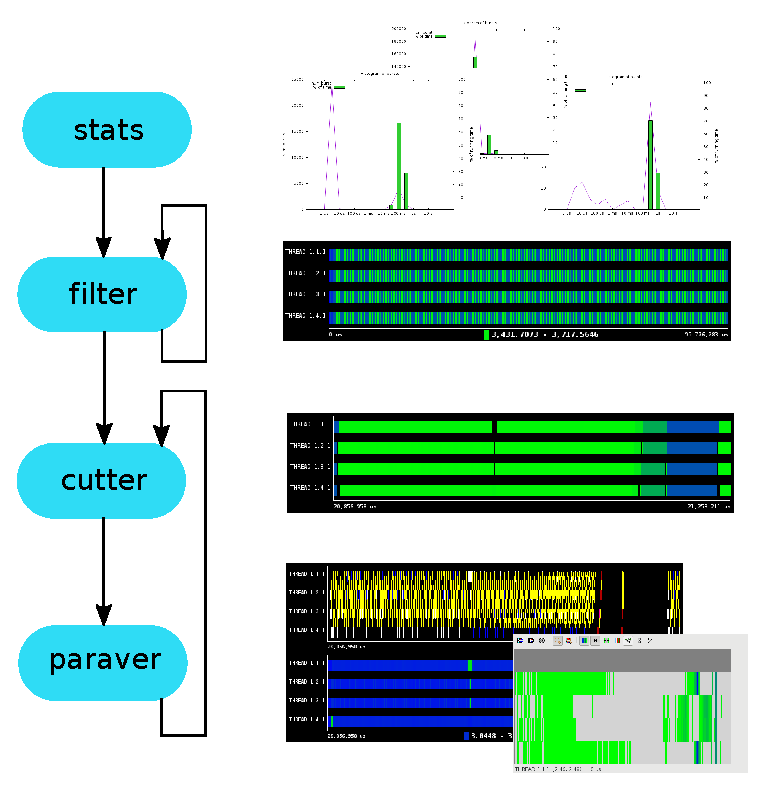
\includegraphics[width=250px]{current_analysis_flow.eps}
\end{figure}


Talk about the BSC performance tools environment and introduce the analysis flow
with and without this proposed tool.

% NOTES
% .- Remember to demonstrate the interarrival time of different calls in the sam
%e loop body tend to be the same.


\bibliography{bibliography}
\bibliographystyle{apalike}
\end{document}
